\documentclass[final,t]{beamer}
\mode<presentation>
{
  \usetheme{MCSposter}
  \usecolortheme{default}
  \usefonttheme[onlymath]{serif}
}
\usepackage[orientation=landscape,size=custom,width=120,height=90,scale=1.3]{beamerposter}
%\usepackage[orientation=landscape,size=a0,scale=1.4]{beamerposter}
\usepackage{pgfpages}
%\pgfpagesuselayout{resize to}[a4paper,landscape,border shrink=5mm]
%\pgfpagesuselayout{resize to}[a0paper,landscape]

% additional settings
\setbeamerfont{itemize}{size=\normalsize}
\setbeamerfont{itemize/enumerate body}{size=\normalsize}
\setbeamerfont{itemize/enumerate subbody}{size=\normalsize}

% additional packages
\usepackage{times}
\usepackage{subfig}
\usepackage{textpos}
\usepackage{wrapfig}
\usepackage{sidecap}
%\usepackage{sfmath} 
\usepackage{amsmath,amsthm,bm,microtype}
\usepackage{siunitx}
\DeclareSIUnit\year{a}
\sisetup{retain-unity-mantissa = false}
\usepackage{exscale}
\usepackage{multicol,multirow}
\usepackage{booktabs}
%\usepackage[english]{babel}
\usepackage[latin1]{inputenc}
\newcommand\todo[1]{{\color{red}\bf [TODO: #1]}}
\usepackage{tikz}
\usetikzlibrary{decorations.pathreplacing}
\usetikzlibrary{shadows,arrows,shapes.misc,shapes.arrows,shapes.multipart,arrows,decorations.pathmorphing,backgrounds,positioning,fit,petri,calc,shadows,chains,matrix}
\usepackage{fancyvrb}
\newcommand\cverb[1][]{\SaveVerb[%
    aftersave={\textnormal{\UseVerb[#1]{vsave}}}]{vsave}}

\bibliographystyle{unsrt-shortauthor}

%\def\newblock{\hskip .11em plus .33em minus .07em} % for natbib and beamer IMPORTANT
\listfiles
\graphicspath{{/home/jed/talks/figures/}{/home/jed/src/aterrel-presentations/figures/}}
% Display a grid to help align images
%\beamertemplategridbackground[1cm]

\newcommand\jedcolor[1]{{}}

\title{\huge Adaptive coarse space construction and nonlinear smoothers for heterogeneous Stokes problems {\normalsize \texttt{DI13C-2434}}}
\author[Jed Brown]{Jed Brown {\texttt{jedbrown@mcs.anl.gov}}, Mark Adams, Matt Knepley, Barry Smith}
\institute[MCS]{Download this poster from \url{http://59A2.org/files/201212-AGUMultigrid.pdf}}

\newcommand{\newt}[1]{\tilde{#1}}
\newcommand{\btab}{\hspace{\stretch{1}}}
\newcommand{\C}{\mathbb{C}}
\newcommand{\N}{\mathbb{N}}
\newcommand{\Q}{\mathbb{Q}}
\newcommand{\R}{\mathbb{R}}
\newcommand{\Rz}{\mathcal{R}}
\newcommand{\RR}{{\bar{\mathbb{R}}}}
\newcommand{\II}{\mathcal{I}}
\newcommand{\Z}{\mathbb{Z}}
\newcommand{\Zp}{\mathbb{Z}_+}
\newcommand{\B}{\mathcal{B}}
\newcommand{\M}{\mathcal{M}}
\newcommand{\LL}{\mathcal{L}}
\newcommand{\PP}{\mathscr{P}}
\newcommand{\ff}{\bm f}
\newcommand{\uu}{\bm u}
\newcommand{\vv}{\bm v}
\newcommand{\ww}{\bm w}
\newcommand{\DD}{D}
\newcommand{\EE}{\mathcal E}
\newcommand{\VV}{\bm{\mathcal{V}}}
\newcommand{\Pspace}{\mathcal{P}}
\newcommand\pfrak{{\mathfrak p}}
\newcommand{\di}{\partial}
\newcommand{\bigO}{\mathcal{O}}
\newcommand{\abs}[1]{\left\lvert #1 \right\rvert}
\newcommand{\bigabs}[1]{\big\lvert #1 \big\rvert}
\newcommand{\norm}[1]{\left\lVert #1 \right\rVert}
\newcommand{\ceil}[1]{\left\lceil #1 \right\rceil}
\newcommand{\floor}[1]{\left\lfloor #1 \right\rfloor}
\newcommand{\dif}{\bigtriangleup}
\newcommand{\ud}{\,\mathrm{d}}
\newcommand{\tcolon}{\!:\!}
\DeclareMathOperator{\sgn}{sgn}
\DeclareMathOperator{\card}{card}
\DeclareMathOperator{\trace}{tr}
\DeclareMathOperator{\sspan}{span}
\renewcommand{\bar}{\overline}
\newcommand{\ed}{\dot{\epsilon}}

% abbreviations
\usepackage{xspace}
\makeatletter
\DeclareRobustCommand\onedot{\futurelet\@let@token\@onedot}
\def\@onedot{\ifx\@let@token.\else.\null\fi\xspace}
\def\eg{{e.g}\onedot} \def\Eg{{E.g}\onedot}
\def\ie{{i.e}\onedot} \def\Ie{{I.e}\onedot}
\def\cf{{c.f}\onedot} \def\Cf{{C.f}\onedot}
\def\etc{{etc}\onedot}
\def\vs{{vs}\onedot}
\def\wrt{w.r.t\onedot}
\def\dof{d.o.f\onedot}
\def\etal{{et al}\onedot}
\makeatother
%%%%%%%%%%%%%%%%%%%%%%%%%%%%%%%%%%%%%%%%%%%%%%%%%%%%%%%%%%%%%%%%%%%%%%%%%%%%%%%%%%%%%%%%%%%%%%%%%%%%%%%%%%%%

% Need to declare these here because newcommand inside a frame is fragile
\newcommand\mgdx{1.9em}
\newcommand\mgdy{2.5em}
\newcommand\mgloc[4]{(#1 + #4*\mgdx*#3,#2 + \mgdy*#3)}
\newcommand{\mglevel}{\ensuremath{\ell}}
\newcommand{\mglevelcp}{\ensuremath{\mglevel_{\mathrm{cp}}}}
\newcommand{\mglevelfine}{\ensuremath{\mglevel_{\mathrm{fine}}}}

\begin{document}
\begin{frame}{} 
  \vspace{-3em}
  \begin{columns}
    \begin{column}{0.31\textwidth}
      \begin{block}{Multigrid in lithosphere and mantle dynamics}
        Heterogeneous Stokes problems appear in various forms throughout geodynamics, often coupled to viscoelasticity, viscoplasticity, and porous media flow.
        As a bottleneck of many high-resolution studies, robust and efficient Stokes solvers are needed.
        These methods are necessarily multilevel and require accurate coarse representations of operators.
        The problems arising in lithosphere dynamics are challenging for standard methods due to multiscale structures creating long-range interaction through thin structures that are difficult to accurately represent using conventional coarse spaces.
        %We incorporate aspects of multigrid, domain decomposition, and multiscale finite element methods to adaptively construct coarse spaces that allow rapid coarsening in smooth regions without sacrificing accuracy in heterogeneous regions.
        %These methods have the additional benefit of working with highly parallel smoothers that can also be used for nonlinear problems.
      \end{block}
      \vspace{-1.5em}
      \begin{block}{Nonlinearity: plasticity and phase change}
        Strong material nonlinearities such as plasticity cause methods based on global linearization, such as Newton and Picard, to require many iterations.
        Nonlinear multigrid avoids global linearization, leading to faster convergence rates when effective nonlinear smoothers are available.
        With a nonlinear smoother, we naturally want to build interpolation and the coarse operator without global assembly of a fine-grid operator.
        Unfortunately, traditional geometric multigrid does not accurately interpolate low-frequency modes and rediscretized coarse operators are notoriously inaccurate in highly heterogeneous cases.
        A subdomain-centric coarse grid construction only involves solving local problems, thus allowing it to be updated only in regions with rapidly-changing nonlinearities.
      \end{block}
      \vspace{-1.5em}
      \begin{block}{Matrix-free for performance}
        \begin{wrapfigure}{r}{0.6\textwidth}
          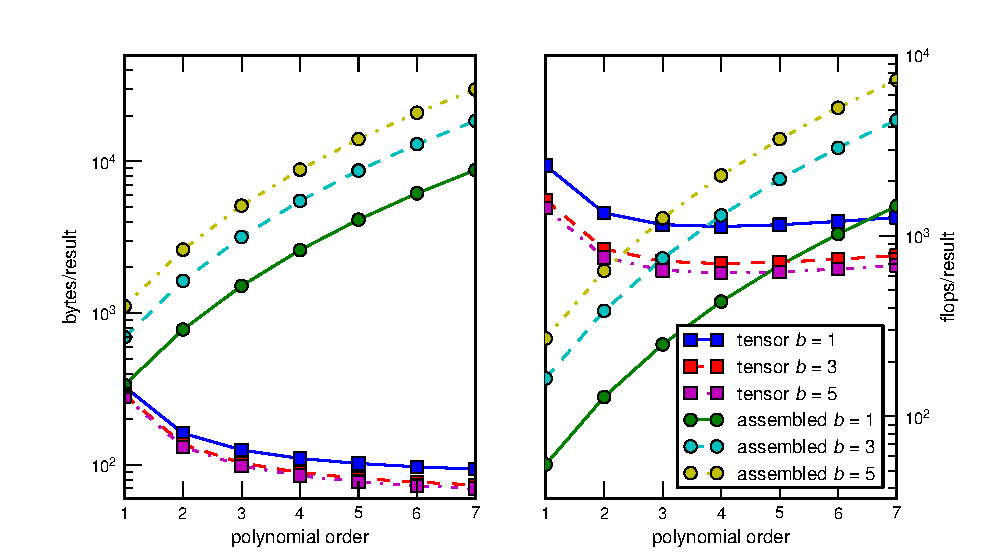
\includegraphics[width=0.58\textwidth]{figures/TensorVsAssembly}
          \caption{Relative cost in memory bandwidth and flops to apply
            linearized PDE operator arising in $p$-version finite
            element discretization of nonlinear PDEs with $b=1,3,5$
            degrees of freedom per node.}\label{fig:TensorVsAssembly}
        \end{wrapfigure}
        Assembled sparse matrices have long been a preferred representation for PDE operators, but are a remarkably poor fit for modern hardware due to memory bandwidth requirements.
        A matrix-vector product computed using an assembled matrix cannot have an arithmetic intensity higher than $1/4$, leaving modern floating point hardware severely under-utilized.
        \begin{table}
          \centering
          \begin{tabular}{lrrr}
            \toprule
            Processor           & BW (GB/s) & Peak (GF/s) & Balanced AI (F/B) \\
            \midrule
            Sandy Bridge 6-core & 21*       & 150         & 7.2                 \\
            Magny Cours 16-core & 42*       & 281         & 6.7                 \\
            Blue Gene/Q node    & 43        & 205         & 4.8                 \\
            % GeForce 9400M       & 21        & 54          & 2.6                 \\
            % GTX 285             & 159       & 1062        & 6.8                 \\
            Tesla M2090         & 120  & 665  & 5.5 \\
            Kepler K20Xm        & 160 & 1310 & 8.2 \\ % http://www.elekslabs.com/2012/11/nvidia-tesla-k20-benchmark-facts.html
            \bottomrule
          \end{tabular}
          \caption{Balanced arithmetic intensity (flops/byte) for several architectures.}\label{tab:BalancedAI}
        \end{table}
      \end{block}
    \end{column}
    %
    \begin{column}{0.31\textwidth}
      \begin{block}{The $\tau$ formulation for multiscale modeling}
        The Full Approximation Scheme is a naturally nonlinear multigrid algorithm that allows flexible incorporation of multilevel information.
        \begin{itemize}
        \item classical formulation: ``coarse grid \emph{accelerates} fine grid solution''
        \item $\tau$ formulation: ``fine grid improves accuracy of coarse grid''
        \item To solve $N u = f$, recursively apply
          \begin{equation*}
            \begin{split}
              \text{pre-smooth} \:\: & \quad \tilde u^h \gets S^h_{\text{pre}}(u^h_0, f^h) \\
              \text{solve coarse problem for $u^H$} \:\: & \quad N^H u^H = \underbrace{I_h^H f^h}_{f^H} + \underbrace{N^H \hat I_h^H \tilde u^h - I_h^H N^h \tilde u^h}_{\tau_h^H} \\
              \text{correction and post-smooth} \:\: & \quad u^h \gets S^h_{\text{post}} \Big( \tilde u^h + I_H^h (u^H - \hat I_h^H \tilde u^h), f^h \Big) \\
            \end{split}
          \end{equation*}
          \begin{tabular}{llll}
            \toprule
            $I_h^H$ & residual restriction & $\hat I_h^H$ & solution restriction \\
            $I_H^h$ & solution interpolation & $f^H = I_h^H f^h$ & restricted forcing \\
            $\{S^h_{\text{pre}},S^h_{\text{post}}\}$ & \multicolumn{3}{l}{smoothing operations on the fine grid} \\
            \bottomrule
          \end{tabular}
        \item At convergence, $u^{H*} = \hat I_h^H u^{h*}$ solves the $\tau$-corrected coarse grid equation
            $N^H u^H = f^H + \tau_h^H$,
          thus $\tau_h^H$ is the ``fine grid feedback'' that makes the coarse grid equation accurate.
        \item $\tau_h^H$ is \emph{local} and need only be recomputed where it becomes stale.
        \end{itemize}
      \end{block}
      \vspace{-2.4em}
      \begin{block}{Subdomain-centric matrix-free coarsening}
        {\bf Objective}: construct robust interpolation and coarse grid operator using only (a) local neighbor information, (b) application of local nonlinear operator, (c) point-block diagonal of principle linearization, and (d) application of triangular distribution operator or splitting~\cite{bkmms2012} for saddle points.
        \begin{enumerate}
        \item Select subdomains to become ``coarse elements'', add minimal stable node set to preliminary set of coarse dofs $C$.
        \item If available, add approximate null space to set of ``low-energy'' modes $B$ that must be approximated accurately.
        \item Use compatible relaxation with point-block preconditioned polynomial smoother to determine deficiencies of initial coarse basis.
        \item Enrich $C$ by adding poorly-converging points.
        \item Optimize energy of local basis functions by computing partition of coarse space $B$ on the boundary, then (approximately) harmonically extending to subdomain interior.
        \item Optionally, use (non-local) bootstrap cycle~\cite{brandt2011bootstrap} to improve $B$.
        \end{enumerate}
      \end{block}
      \vspace{-2.4em}
      \begin{block}{Low-communication cycling}
            \begin{wrapfigure}{r}{0.45\textwidth}
              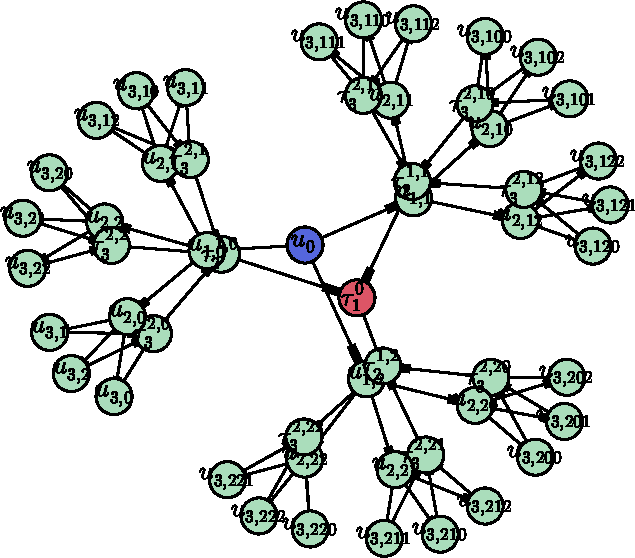
\includegraphics[width=0.4\textwidth]{figures/MG/TauDeps.pdf}
            \end{wrapfigure}
            The $\tau$ formulation removes communication from all levels except the coarsest.
            Instead of starting and ending on the fine grid, a cycle starts and ends on the coarse grid.
            The figure shows the dependency graph of 3-level multigrid cycle that computes the correction $\tau_1^0$ (red) on the coarse grid equation starting with coarse grid state $u_0$ (blue).
            A traditional multigrid cycle which has ``horizontal'' dependencies at every level.
      \end{block}
    \end{column}
    %
    \begin{column}{0.31\textwidth}
      \begin{block}{Multiscale compression and decompression}
        \begin{tikzpicture}
          [scale=0.7,every node/.style={scale=0.7},
          >=stealth,
          restrict/.style={thick,double},
          prolong/.style={thick,double},
          cprestrict/.style={green!50!black,thick,double,dashed},
          control/.style={rectangle,red!40!black,draw=red!40!black,thick},
          mglevel/.style={rounded rectangle,draw=blue!50!black,fill=blue!20,thick,minimum size=6mm},
          checkpoint/.style={rectangle,draw=green!50!black,fill=green!20,thick,minimum size=6mm},
          mglevelhide/.style={rounded rectangle,draw=gray!50!black,fill=gray!20,thick,minimum size=6mm},
          tau/.style={text=red!50!black,draw=red!50!black,fill=red!10,inner sep=1pt},
          crelax/.style={text=green!50!black,fill=green!10,inner sep=0pt}
          ]
          \begin{scope}
            \node[mglevel] (fine0) at \mgloc{0}{0}{4}{-1} {\mglevelfine};
            \node[mglevel] (finem1down0) at \mgloc{0}{0}{3}{-1} {};
            \node[mglevel] (cp1down0) at \mgloc{0}{0}{2}{-1} {$\mglevelcp+1$};
            \node[mglevel] (cpdown0) at \mgloc{0}{0}{1}{-1} {\mglevelcp};
            \node[mglevel] (coarser0) at \mgloc{0}{0}{0}{0} {\ldots};

            \node[mglevelhide] (cpup0) at \mgloc{0}{0}{1}{1} {};
            \node (cp1up0) at \mgloc{0}{0}{2}{1} {};

            \node (cpdown1) at \mgloc{4em}{0}{1}{-1} {};
            \node[mglevelhide] (coarser1) at \mgloc{4em}{0}{0}{1} {\ldots};
            \node[mglevel] (cpup1) at \mgloc{4em}{0}{1}{1} {\mglevelcp};
            \node[mglevel] (cp1up1) at \mgloc{4em}{0}{2}{1} {$\mglevelcp+1$};
            \node[mglevel] (finem1up1) at \mgloc{4em}{0}{3}{1} {};
            \node[mglevel] (fine1) at \mgloc{4em}{0}{4}{1} {\mglevelfine};

            \draw[->,restrict,dashed] (fine0) -- (finem1down0);
            \draw[->,restrict] (finem1down0) -- (cp1down0);
            \draw[->,restrict] (cp1down0) -- (cpdown0);
            \draw[->,restrict,dashed] (cpdown0) -- (coarser0);
            \draw[->,prolong,dashed] (coarser0) -- (cpup0);
            \draw[->,prolong,dashed] (cpup0) -- (cp1up0);

            \draw[->,restrict,dashed] (cpdown1) -- (coarser1);
            \draw[->,prolong,dashed] (coarser1) -- (cpup1);
            \draw[->,prolong] (cpup1) -- (cp1up1);
            \draw[->,prolong] (cp1up1) -- (finem1up1);
            \draw[->,prolong,dashed] (finem1up1) -- (fine1);

            \node[checkpoint] at (4em + \mgdx*4,\mgdy) (cp) {CP};
            \draw[>->,cprestrict] (fine1) -- node[below,sloped] {Restrict} (cp);

            \node[left=\mgdx of fine0] (bnanchor) {};
            \node[control,fill=red!20] at (1.1*\mgdx,3*\mgdy) {Solve $F(u^n;b^n) = 0$};
            \node[mglevel,right=of fine1] (finedt) {next solve};
            \draw[->, >=stealth, control] (fine1) to[out=20,in=170] node[above] {$b^{n+1}(u^n,b^n)$} (finedt);
            \draw[->, >=stealth, control] (bnanchor) to[out=45,in=155] node[above] {$b^n$} (fine0);

            % Recovery process
            \begin{scope}[xshift=8*\mgdx]
              \node[checkpoint] (rcp) at \mgloc{0}{0}{0}{0} {CP};
              \node[mglevel] (r0a) at \mgloc{0}{\mgdy}{0}{0} {CR};
              \node[mglevel] (r1a) at \mgloc{0}{\mgdy}{1}{1} {};
              \node[mglevel] (r0b) at \mgloc{2*\mgdx}{\mgdy}{0}{0} {CR};
              \node[mglevel] (r1b) at \mgloc{2*\mgdx}{\mgdy}{1}{1} {};
              \node[mglevel] (r2b) at \mgloc{2*\mgdx}{\mgdy}{2}{1} {\mglevelfine};
              \node[mglevel] (r1c) at \mgloc{6*\mgdx}{\mgdy}{1}{-1} {};
              \node[mglevel] (r0d) at \mgloc{6*\mgdx}{\mgdy}{0}{0} {CR};
              \node[mglevel] (r1d) at \mgloc{6*\mgdx}{\mgdy}{1}{1} {};
              \node[mglevel] (r2d) at \mgloc{6*\mgdx}{\mgdy}{2}{1} {\mglevelfine};

              \draw[-,prolong,green!50!black] (rcp) -- (r0a);
              \draw[->,prolong] (r0a) -- (r1a);
              \draw[->,restrict] (r1a) -- (r0b);
              \draw[->,restrict] (r0b) -- (r1b);
              \draw[->,restrict,dashed] (r1b) -- (r2b);
              \draw[->,restrict,dashed] (r2b) -- (r1c);
              \draw[->,restrict] (r1c) -- (r0d);
              \draw[->,restrict] (r0d) -- (r1d);
              \draw[->,restrict,dashed] (r1d) -- (r2d);

              \foreach \smooth in {finem1down0, cp1down0, cpdown0, coarser0,
                cpup1, cp1up1, finem1up1,
                r0b,r1c,r0d,r1d} {
                \node[above left=-5pt of \smooth.west,tau] {$\tau$};
              }
              \node[rectangle,fill=none,draw=green!50!black,thick,fit=(rcp)(r2d)] (recoverbox) {};
              \node[rectangle,draw=green!50!black,fill=green!20,thick,minimum size=6mm,above={0cm of recoverbox.south east},anchor=south east] (recover) {FMG Decompression};
            \end{scope}
            \node (notation) at (2*\mgdx,5*\mgdy) {
              \begin{minipage}{18em}\small\sf
                \begin{itemize}\addtolength{\itemsep}{-5pt}
                \item checkpoint converged coarse state
                \item recover using FMG anchored at $\mglevelcp+1$
                \item needs only $\mglevelcp$ neighbor points
                \item $\tau$ correction is local
                \end{itemize}
              \end{minipage}
            };
          \end{scope}
        \end{tikzpicture}
        \begin{itemize}
        \item Fine state $u^{h*}$ recovered \emph{locally} from converged coarse state $u^{H*} = \hat I_h^H u^{h*}$
        \item Normal multigrid cycles visit all levels moving from $n \to n+1$
        \item FMG recovery only accesses levels finer than $\ell_{CP}$
        \item Only neighborhood of desired region needed during decompression
        \item Lightweight checkpointing for transient adjoint computation
        \item Postprocessing applications, e.g., in-situ visualization at high temporal resolution in part of the domain
        \end{itemize}
      \end{block}      
      \vspace{-2.4em}
      \begin{block}{Local decompression and resilience}
        \begin{tikzpicture}
          [scale=1,every node/.style={scale=1},
          >=stealth,
          control/.style={rectangle,rounded corners,draw=blue!50!black,fill=blue!20,thick,minimum width=5em},
          essential/.style={rectangle,rounded corners,draw=red!50!black,fill=red!20,thick,minimum width=5em},
          ephemeral/.style={rectangle,rounded corners,draw=gray!50!black,fill=gray!20,thick,minimum width=5em},
          statebox/.style={rectangle,draw=green!50!black,thick},
          statetitle/.style={rectangle,draw=green!50!black,fill=green!20,thick},
          storebox/.style={rectangle,draw=},
          rightbrace/.style={decorate,decoration={brace,amplitude=1ex,raise=4pt}},
          leftbrace/.style={decorate,decoration={brace,amplitude=1ex,raise=4pt,mirror}}
          ]
          \scriptsize
          \node[control,minimum width=8em] (progcontrol) {control};
          \node[essential,below=2pt of progcontrol.south,rectangle split,rectangle split parts=2,rectangle split horizontal,minimum width=12em] (progessential) {essential \nodepart{two} coarse};
          \node[ephemeral,minimum width=8em,below=2pt of progessential.south] (progephemeral) {ephemeral};
          \node[statebox,fit=(progcontrol)(progessential)(progephemeral)] (progbox) {};
          \node[above=0pt of progbox.north,anchor=south] {\textbf{program $n=0$}};

          \node[control,right=9em of progcontrol] (storecontrol) {control};
          \node[essential,below=2pt of storecontrol.south] (storeessential) {essential};
          \node[essential,minimum width=4em,below=6pt of storeessential.south, double copy shadow] (storecoarse) {coarse};
          \node[statebox,decorate,decoration={bumps,mirror},fit=(storecontrol)(storecoarse)] (storebox) {};
          \node[above=1pt of storebox.north,anchor=south] {\textbf{storage}};

          \node[control,right=7em of storecontrol] (reccontrol) {control};
          \node[essential,below=2pt of reccontrol.south] (recessential) {essential};
          \node[statebox,fit=(reccontrol)(recessential)] (recbox) {};
          \node[above=0pt of recbox.north,anchor=south] {\textbf{restored $n=0$}};

          \node[control,right=6em of reccontrol] (donecontrol) {control};
          \node[essential,below=2pt of donecontrol.south] (doneessential) {essential};
          \node[ephemeral,below=2pt of doneessential.south] (doneephemeral) {ephemeral};
          \node[statebox,fit=(donecontrol)(doneephemeral)] (donebox) {};
          \node[above=0pt of donebox.north,anchor=south] {\textbf{recovered $n=N$}};

          \draw[decorate,decoration={brace,amplitude=1ex,raise=4pt}] ($(progcontrol.north east) + (3pt,0)$) -- ($(progephemeral.north east) + (3pt,0)$) node[midway,xshift=1ex] (progbrace) {};
          \draw[leftbrace] ($(storecontrol.north west) - (4pt,0)$) -- ($(storeessential.south west) - (4pt,0)$) node[midway,xshift=-1ex] (storebrace) {};
          \draw[rightbrace] ($(storecontrol.north east) + (4pt,0)$) -- ($(storeessential.south east) + (4pt,0)$) node[midway,xshift=1ex] (storerbrace) {};
          \draw[->,shorten >=4pt,shorten <=4pt] (progbrace) -- (storebrace) node[midway,above] (midarrow) {MPI/BLCR};

          \node[below=1.4em of midarrow,essential,draw=red!50!gray!70,fill=red!10] (coarserun) {};
          \draw[->,dashed,shorten >=14pt,shorten <=4pt] (coarserun) |- (storecoarse) node [near start,below,yshift=-3pt] {\scriptsize $n=1,2,\dotsc,N$};
          \draw[->,shorten >=4pt,shorten <=4pt] (storerbrace) -- (recbox.west) node[midway,above,text width=5em,align=center] (midarrow) {restart failed ranks};
          \draw[->,shorten >=5pt,shorten <=4pt] (recessential.east) -- (doneessential) node[midway,above,text width=5em,align=center] (fmgrecover) {FMG recovery};
          \draw[->,dashed,shorten >=1pt,shorten <=3pt] ($(storecoarse.east) + (1em,0)$) -| (fmgrecover) node[midway,below,xshift=-1em] {\scriptsize $n=1,2,\dotsc,N$};
          \draw[->,dashed,shorten >=3pt,shorten <=3pt] (donecontrol.east) -| ($(donecontrol.east) + (3ex,0)$) |- (doneephemeral.east) node[midway,right,text width=4em] {\cverb|malloc| at $n=0$};
        \end{tikzpicture}
        \begin{description}
        \item[control] contains program stack, solver configuration, etc.
        \item[essential] program state that cannot be easily reconstructed: time-dependent solution, current optimization/bifurcation iterate
        \item[ephemeral] easily recovered structures: assembled matrices, preconditioners, residuals, Runge-Kutta stage solutions
        \end{description}
        \begin{itemize}
        \item Essential state at time/optimization step $n$ is \alert{inherently globally coupled} to step $n-1$ (otherwise we could use an explicit method)
        \item \emph{Coarse} level checkpoints are orders of magnitude smaller, but allow rapid recovery of essential state
        \item FMG recovery needs only \alert{nearest neighbors}
        \end{itemize}
      \end{block}
      \vspace{-2.4em}
      \begin{block}{Status}
        Proof-of-concept compatible relaxation and subdomain coarsening implemented using PETSc, similar robustness to modern smoothed aggregation.
        Low-communication implementation and use of more efficient data structures for local decomposition in progress.
        Merging subdomain-centric approach with PCGAMG (algebraic multigrid infrastructure), along with accessible user hooks for customization.
      \end{block}
      \vspace{-2.4em}
      \begin{block}{References}
        \scriptsize
        \nocite{brandt1994multigrid,bkmms2012}
        \begin{minipage}{\textwidth}
          \begin{multicols}{2}
            \bibliography{$HOME/jedbib/jedbib,$PETSC_DIR/src/docs/tex/petsc,$PETSC_DIR/src/docs/tex/petscapp}
          \end{multicols}
        \end{minipage}
      \end{block}
    \end{column}
  \end{columns}
\end{frame}
\end{document}

        % Recursive application of a technique called \emph{segmental refinement}, in which the fine grid state is populated on the fly from the coarser grid followed by smoothing, permits solution of problems using only poly-logarithmic memory, provided that the right hand side and coefficients are similarly compressible.
        % For highly heterogenous problems, the constants associated with this aggressive memory reduction become large, and we have to choose which ingredients are most crucial to a robust multigrid cycle.
        % \begin{description}
        % \item[Solution state] is small and frequently needed in complete form due to coupling to other equations and time-dependence.
        %   It is relatively expensive to reconstruct on the fly, especially on multiple coarse levels.
        % \item[Grid transfer operators] (coarse basis functions) are a critical ingredient for robust multigrid and also expensive to reconstruct in each visit.
        % \item[Coarse operators] provide a systematic compression of fine-scale heterogeneity.
        %   With a fast coarsening rate, coarse grid operators are relatively affordable.
        % \item[Fine grid operators] typically consume significantly more memory than the rest of the multigrid hierarchy, are performance-limited by memory bandwidth, and too expensive to reassemble for highly nonlinear problems.
        % \end{description}

%%%%%%%%%%%%%%%%%%%%%%%%%%%%%%%%%%%%%%%%%%%%%%%%%%%%%%%%%%%%%%%%%%%%%%%%%%%%%%%%%%%%%%%%%%%%%%%%%%%% 
%%% Local Variables: 
%%% mode: latex
%%% TeX-PDF-mode: t
%%% End: 


